\documentclass[dutch, 11pt]{report}
%\documentclass[dutch, 11pt]{scrartcl}

\newbox\one
\newbox\two
\long\def\loremlines#1{%
	\setbox\one=\vbox {%
		\lipsum%
	}
	\setbox\two=\vsplit\one to #1\baselineskip
	\unvbox\two}


%\newcommand{\Course}{Multimediatechnieken}
%\newcommand{\CourseShort}{MMT}
\newcommand{\Course}{Algoritmen en Datastructuren 2}
\newcommand{\CourseShort}{AD2}

\usepackage[dutch, english]{babel}
\usepackage{graphicx}
\usepackage{subfig}
\usepackage{lipsum}
\usepackage[utf8]{inputenc}
\usepackage{float}
\usepackage{hyperref}
\usepackage{graphicx}
\graphicspath{ {./Images/} }

%opening
\title{Verslag project: semi-splaybomen}
\author{\Course\\
Victor Matthijs}
\date{27-10-2019}

\begin{document}

\maketitle

\section*{Inleiding}
In dit project gaan we een geparametriseerde variant op de semi-splaybomen uit de cursus implementeren en bekijken wat de theoretische en experimentele performantie van deze variant is in functie van de parameter.


\section*{Opgave}
Bij de semi-splaybomen zoals ze in de cursus beschreven staan, worden op het pad naar de wortel steeds drie toppen genomen, en dit deelpad wordt vervangen door een volledige binaire boom met drie toppen. De bedoeling van dit project is om een variant te implementeren, waarbij de splaygrootte k(het aantal toppen dat wordt samengenomen in een splaystap) kan aangepast worden, maar we stellen wel dat dit steeds minstens drie moet zijn. Vervolgens vervangen we dit deelpad door een perfect gebalanceerde boom, dus met diepte log(k). Als de parameter k van de vorm 2n - 1 is met n een natuurlijk getal, dan is dit een volledige binaire boom. Als k echter niet van deze vorm is, dan zijn er meerdere mogelijke bomen. Je bent hier vrij om zelf een keuze te maken (eventueel gebaseerd op experimenten), maar kies wel een boom die zo goed mogelijk gebalanceerd is.

\section*{Theoretische vragen}
Het theoretische gedeelte is even belangrijk als de implementatie, dus besteed er voldoende tijd aan. Geef een duidelijke beschrijving met pseudocode van je algoritmes. Implementatiedetails en Java-specifieke dingen horen hier niet thuis. Zorg ervoor dat je bewijzen volledig en correct zijn. Je mag gebruik maken van resultaten uit de cursus. Vermeld altijd welke eigenschappen je gebruikt.\newpage

\subsection*{1. Geef een (exacte) uitdrukking voor het aantal mogelijke vormen dat het pad met k toppen kan hebben dat tijdens een splaystap vervangen wordt door een boom.}

Vooraleer een exacte uitdrukking te geven voor het aantal mogelijke vormen ben ik eerst beginnen nadenken over het triviale geval met $k=3$, zoals eerder in de les gezien is. Wanneer het aantal toppen k gelijk is aan 3 krijgen we onderstaande mogelijkheden.\newline

\begin{figure}[h]
\caption{3 Toppen Voorbeeld}
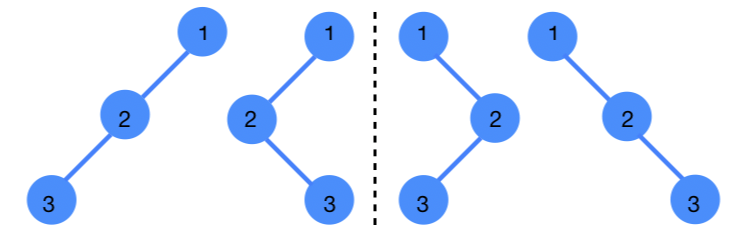
\includegraphics[width=\textwidth]{3_Toppen}
\centering
\end{figure}

Zoals we in dit voorbeeld met $k=3$ kunnen zien, hebben we een even aantal mogelijkheden, telkens is de ene helft een spiegeling van de andere helft. We kunnen ons nu echter afvragen of dit ook het geval is voor grotere waardes van k.

Wanneer we kijken naar de mogelijkheden van $k=4$, kunnen we besluiten dat ook hier het aantal even is. Net als bij $k=3$ is ook hier een stippellijn getrokken om aan te geven dat we te maken hebben met spiegeling. Wanneer men 4 toppen als een semi splay pad neemt dan bekomt men 8 verschillende mogelijkheden. (bijlage, figuur 4)

Wanneer we $k$ blijven incrementeren, kunnen we het volgende besluiten. De wortel van het pad (in de figuren aan geduid met nummer 1) zullen steeds maar één mogelijkheid hebben. We kunnen dit ook als volgt formuleren: "De wortel blijft op een centrale positie". Echter alle andere toppen, dus $k - 1$ toppen, kunnen op twee posities worden geplaatst. Zowel links van hun ouder als rechts van hun ouder is een geldige positie. Door deze redenering om te zetten in een bruikbare formule krijgen we het volgende
$$
k\ toppen => 2^{k-1}\ mogelijke\ vormen
$$

\begin{figure}[h]
\caption{Vraag 2}
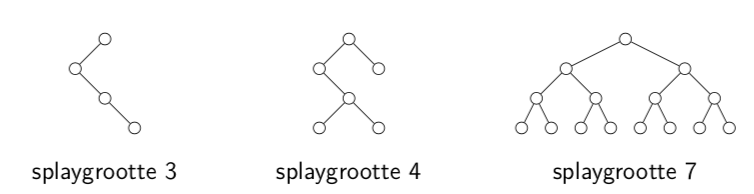
\includegraphics[width=\textwidth]{Vraag2}
\centering
\end{figure}
\newpage

\subsection*{2. Geef voor elk van de bomen en splaygroottes (figuur 3) een reeks van toevoeg- en opzoekbewerkingen die resulteren in een boom isomorf aan deze boom, of bewijs dat dit niet kan. Let op: geen verwijderbewerkingen}
\subsubsection*{Splaygrootte 3}
Als we naar de doelplaatsen kijken van alle toppen (zie figuur 3,a), dan kunnen we het volgende opmerken: $A > D > C > B$.
In welke volgorde we de getallen/toppen ook toevoegen, na de eerste 3 toevoegbewerkingen zullen we altijd de volgende situatie bekomen (zie figuur 3,b). De wortel kan op dit moment nooit top A of B bevatten, maar enkel C of D. A en B kunnen hier niet omdat deze toppen de grootste en de kleinste zijn en wanneer men een semisplay bewerking met 3 toppen gaat uitvoeren, dan zullen A en B altijd kinderen van de nieuwe binaire boom zijn met drie toppen. Een opzoekbewerking heeft hier echter ook nog geen nut, want geen enkel pad is lang genoeg om een semisplay bewerking op toe te passen. \newline

\begin{figure}%
    \centering
    \subfloat{{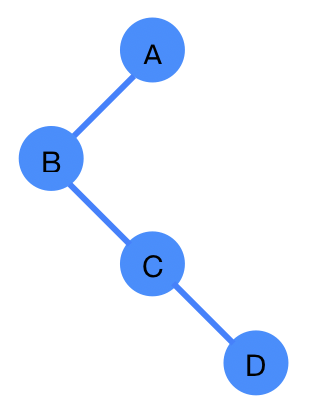
\includegraphics[width=5cm]{BeginSituatie} }}%
    \qquad
    \subfloat{{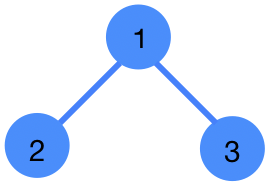
\includegraphics[width=5cm]{3_Toevoeg} }}%
    \caption{}%
\end{figure}

De enige volgende stap is het toevoegen van het laatste element, deze zal altijd een semisplay bewerking veroorzaken binnen de boom. Ook bij deze semisplay bewerking kunnen we de vorige opmerking herhalen. De toppen A en B (grootste en kleinste sleutel van de 4) zullen nooit in de wortel staan. De twee mogelijke bomen staan weergegeven in de bijlage (figuur 5). Na het toevoegen van alle toppen hebben we dus te maken met deze twee mogelijkheden. De enige mogelijke bewerking is nu om een opzoeking te doen op de laagste top, want enkel op de dit pad zal er kunnen gesplayed worden. Echter kunnen we besluiten dat de ene opzoekingsbewerking zal resulteren in de andere boom en omgekeerd. 
We kunnen dus besluiten dat we geen reeks van toevoeg- en opzoekbewerkingen kunnen opstellen die resulteren in een boom die isomorf is aan de boom in figuur 4a.

\subsubsection*{Splaygrootte 4}
Ook voor deze boom (figuur 3, b) kunnen we inzien dat er geen reeks van toevoeg- en opzoekbewerkingen bestaat om het gegeven resultaat te bekomen. De enige twee mogelijke resultaten na het uitvoeren van een semisplay bewerking met splaygrootte 4 worden weergegeven in figuur 5. We kunnen zien dat deze structuur niet voorkomt in de gegeven eindboom. Deze eindboom kan men enkel bereiken door minstens een keer een semisplay stap met grootte 4 uitgevoerd te hebben, dus hieruit kunnen we besluiten dat er geen reeks is om een boom isomorf aan de eindboom te construeren.
\subsubsection*{Splaygrootte 7}
Voor de derde deelvraag is het gemakkelijk in te zien dat er een reeks van toevoeg- en opzoekbewerkingen bestaat die resulteert in de startboom met splaygrootte 7 (figuur 3). \newline
Wanneer men de volgende reeks van getallen toevoegt, dan zal men tot de gegeven boom komen (zie bijlage, figuur 6).
De reeks geldt als volgt $8, 4, 12, 2, 6, 10, 14, 1 , 3, 5, 7, 9, 11, 13, 15$. We zien duidelijk dat we op deze boom bij geen enkele toevoegbewerking een splay operatie hebben moeten uitvoeren, dit komt echter omdat geen pad lang genoeg is.\newline
We kunnen hieruit dus besluiten dat de bovenstaande reeks van toevoegbewerkingen resulteert in een boom isomorf aan de beginboom.

\subsection*{3. Bepaal en bewijs de gemiddelde complexiteit van een bewerking in een reeks van n bewerkingen op een initieel lege semi-splayboom met splaygrootte 7.}

\subsection*{4. Geef een zo efficient mogelijk algoritme om een splaypad met k toppen te vervangen door een perfect gebalanceerde deelboom.}
Het algoritme voor het vervangen van een pad met k toppen door een perfect gebalanceerde boom staat beschreven in de code door 4 verschillende deelfuncties. De verschillende functies en hun verband met elkaar wordt hieronder verduidelijkt:
\begin{itemize}
	\item $semiSplayStep$: Dit is de eerste functie die wordt opgeroepen voor het vervangen van een pad door een perfecte deelboom. We geven hier een parameter mee met alle toppen in volgorde zoals ze op het pad voorkomen. De lengte van een $splaystap k$ werd al meegegeven met de constructor van de boom. Deze functie zal gebruik maken van een stack, $nodeStack$,  om te bepalen hoeveel keer een pad de semi-splay bewerking moet uitvoeren om tot een correcte oplossing te komen. Zolang er genoeg toppen op de stack staan om een semisplay bewerking uit te voeren zal men een $splayStepList$ construeren met de volgende $k$ toppen die een perfecte deelboom moeten vormen. Hier wordt vervolgens gebruik gemaakt van de functie $getAllOuterTrees$, zoals beschreven hieronder. Na het opslaan van alle buitenbomen op het pad met lengte $k$ wordt de functie $recSemiSplay$ opgeroepen. Na het opbouwen van de nieuwe deelboom met $k$ toppen zal de functie $addAllOuterTrees$ worden opgeroepen om de deelbomen weer op de juiste plaats toe te voegen. Als laatste stap zal deze functie de wortel van de nieuwe deelboom terug toevoegen aan de stack. Als deze stack nu minstens $k$ toppen bevat dan zal het proces voor het opstellen van een perfect gebalanceerde deelboom opnieuw beginnen. Stel dat de stack minder dan $k$ toppen heeft dan wordt de laatste nieuwe deelboom op de juist plaats in de boom terug geplaatst en zal de functie eindigen. We zien dus dat deze functie een pad met $k$ toppen zal omvormen tot een perfect gebalanceerde deelboom binnen de oorspronkelijke boom.
	\item $getAllOuterTrees$: Zoals de naam al weergeeft zal deze functie alle $k+1$ buitenbomen van een pad met lengte $k$ verzamelen en terug geven als een array van toppen. Het pad wordt overlopen, beginnend met de wortel, en telkens wordt er nagegaan of er een buitenboom aanwezig is. Zo ja dan wordt deze op de juiste plaats in de array opgeslaan zodat men die later weer op de correcte plaats kan toevoegen bij de nieuwe perfecte deelboom. Als er geen buitenboom is bij een top, dan zal $null$ worden bewaard op de juiste plaats in de array. Deze functie geeft alle buitenbomen terug in de juiste volgorde, van de kleinste tot de grootste top.
	\item $recSemiSplay$: Deze functie zal recursief een correcte binaire boom opbouwen met $k$ toppen. De enige parameter bij deze recursieve functie is een lijst van de $k$ toppen gesorteerd in stijgende volgorde. De functie zal nu telkens het element op de middelste positie van de lijst nemen en dit als nieuwe wortel gebruiken bij de nieuwe deelboom. De kinderen van deze nieuwe wortel worden recursief bepaalt door twee keer de functie op te roepen, telkens met een kleinere lijst van toppen. Het linkerkind wordt opgebouwd met de lijst van alle toppen kleiner dan de nieuwe wortel, het rechterkind met een lijst van kinderen groter dan de wortel. Zoals te zien is in de code zal een lijst met slechts één element, enkel een wortel bevatten en zullen de kinderen van deze wortel op $null$ worden gezet. Hier worden dan later de buitenbomen weer correct aan toegevoegd. Een lijst met slechts twee toppen zal worden omgezet in een deelboom met een wortel en een linkerkind, het rechterkind wordt op $null$ gezet, zo zien we dat we altijd een perfect gebalanceerde deelboom zullen krijgen bij het uitvoeren van deze functie.
	\item $addAllOuterTrees$: Deze functie zal alle $k+1$ buitenbomen op de correcte plaats in de nieuwe gebalanceerde deelboom terugplaatsen. De functie zal alle toppen van de nieuwe deelboom in stijgende volgorde overlopen. Telkens wanneer een top een leeg kind heeft zal de juiste buitenboom worden gekozen uit de array van buitenbomen. Na het uitvoeren van deze functie is het pad met $k$ toppen vervangen door een een perfect gebalanceerde deelboom met $k$ toppen.
\end{itemize}

\subsection*{5. Bepaal en bewijs de complexiteit van het algoritme uit de vorige vraag.}


\newpage
\section*{Bespreking implementatie}
Voor dat we de functies uit de klasse SemiSplay gaan bespreken, is het eerste interessant om aan te halen dat er in dit project ook een klasse Node gebruikt wordt. Deze klasse wordt doorheen heel het project gehanteerd om de boom gemakkelijker te kunnen voorstellen. Zoals te zien is in de code bevat de klasse Node 3 velden, de waarde van de node zelf met daarnaast een verwijzing naar zowel zijn linker als zijn rechter kind. Deze twee verwijzingen kunnen natuurlijk ook null zijn, dan heeft deze top in de boom geen kinderen en is het een blad. Hieronder leggen we een voor een de functies uit die in de klasse SemiSplay terug te vinden zijn.

\subsection*{A) Functie: constructor SemiSplayTree}
Als eerste functie in de klasse SemiSplayTree hebben we de constructor met parameter Splaysize(de grootte van het path) , deze constructor zal de velden van de klasse initialiseren op de juiste waardes. We definiëren de root van de boom op Null en daarop volgende zetten we het veld Size op 0. (zie functie Size)

\subsection*{B) Functie: add node}
Als tweede functie in de klasse semiSplayTree hebben we de toevoegoperatie. Deze functie neemt een Comparable als argument en zal deze op de juiste plaats in de boom toevoegen. We geven False terug indien de boom dit element al bevat. Binnenin deze functie gaan we simpel te werk, we gaan eerst na of de wortel van onze boom al een Node bevat. Indien dit niet het geval is kunnen we gemakkelijk de nieuwe Node toevoegen en stopt onze operatie. Indien dit niet zo is maken we handig gebruik van de functie compareTo die we hebben overschreven(override) in de klasse Node. Deze compareTo functie zal twee Nodes vergelijken en een integer terug geven. Aan de hand van dit getal zakken we dieper af in de boom tot op een bepaald punt. Hier zijn er nu twee mogelijkheden, ofwel zal de compareTo 0 terug geven en dit wijst erop dat het element al in de boom zat, we geven False terug. Als de compareTo een element verschillende van 0 terug geeft, kunnen we de nieuwe node op de correcte plaats toevoegen in de boom door de juiste pointers te updaten. Gedurende alle vergelijkingen houden we ook een lijst bij met alle toppen op het pad die we overlopen hebben. Deze lijst wordt dan gebruikt bij de semisplaystep functie (zie verder).

\subsection*{C) Functie: remove node}
De functie remove werkt zoals beschreven in de cursus. We zoeken eerst het te verwijderen element op in de boom. Als we dit element niet vinden, dan returns we false. Als het element wel in de boom zit hebben we verschillende mogelijkheden. Het element kan een leaf node zijn, dan kunnen we deze gewoon verwijderen in de boom en updaten we de kinderen van de parent correct. Als de node geen leaf is, maken we gebruik van het volgende algoritme: neem het kleinste element uit de rechter deelboom en switch de twee elementen, men kan nu de leaf weer verwijderen zoals hiervoor. Er is een functie getMinNode geschreven om het kleinste element uit een deelboom te halen, deze functie maakt ha dig gebruik van het feit dat het kleinste element altijd op de meest linkse positie staat in de deelboom. In de verwijder functie werd ook gekozen om enkele if-else structuren te gebruiken om tot de juiste conclusies te komen tijdens het algoritme.

\subsection*{D) Functie: size}
Deze functie is heel eenvoudig te bespreken, bij elke toevoegbewerking incrementeren we het veld size, analoog decrementeren we bij elke removebewerking het veld. Dit zal dus altijd tot de goede oplossing leiden wanneer er wordt gevraagd om de grootte van de boom terug te geven. Indien het gebruik van zo een veld toch niet wordt toegelaten staat er in comments alsnog een andere implementatie om de size van een boom te berekenen.

\subsection*{E) Functie: contains node}
De volgende functie in het bestand is de contains functie, deze functie zal checken of een gegeven Node in de boom aanwezig is of niet. Deze implementatie van de functie is eigenlijk hetzelfde principe als de toevoeroperatie, maar in plaats van het daadwerkelijk toevoegen van de node geven we nu enkel terug of de node in de boom aanwezig is. We maken ook hier opnieuw gebruik van de compareTo functie om twee Nodes met elkaar te vergelijken. In de implementatie is duidelijk dat wanneer de while-loop is afgelopen en er nog steeds geen Node is gevonden met dezelfde waarde dan wordt False teruggegeven.

\subsection*{F) Functie: depth of a tree}
Deze functie berekend de diepte van de boom, hier wordt er gewerkt met een Depth-First search approach op het probleem. De functie maakt gebruik van een hulpfunctie die we iteratief oproepen om de diepte van de boom te berekenen. De MaxDepth functie zal iteratief de diepte van eerst zijn linker kind vragen en daarna dat van zijn rechter kind. Hierna bepalen we het maximum van deze twee en voegen we daar 1 bij toe, voor de top zelf mee te tellen.

\subsection*{G) Iterator}
Een van de laatste functie dat we geïmplementeerd hebben is de iterator. Hier hebben de klasse iterator overschreven zodat we onze eigen implementatie konden gebruiken bij sommige belangrijke methoden. De constructor wordt overschreven zodat de implementatie gebruik kan maken van een stack. Deze stack wordt dan gebruikt om de toppen in stijgende volgorde te overlopen. We hebben ervoor gekozen om een stack te gebruiken omdat dit de methodes next en hasNext gemakkelijker maakt. In de code is ook te zien dat de methode remove niet wordt geïmplementeerd, hiervoor gebruiken we de NoSuchMethodException, als we deze methode niet implementeerden dan gaf java een compile error.

\subsection*{H) Functie: semiSplayStep}
Deze functie werd geïmplementeerd in het tweede deel van het project. Hier is het dus de bedoeling dat we de semisplay operatie uitschrijven, zodat na elke bewerking deze kan uitgevoerd worden. Uit de opgave volgt ook dat de splay lengte van het path als een variabele moet meegegeven worden. Dit gebeurd echter al in de constructor van de semiSplay klasse. Zoals in de cursus beschreven staat (pagina 15) wordt de semisplay operatie op meerdere plaatsen in de code uitgevoerd:

\begin{itemize}
	\item Add: De semisplay operatie wordt uitgevoerd op het pad naar de node die men juist heeft toegevoegd aan de boom. Als de node al in de boom zat dan wordt het alsnog het pad tot de node gebruikt om een semisplay operatie uit te voeren.
	\item Remove: Als de top wordt gevonden dan voeren we de verwijder operatie uit zoals beschreven hierboven en dan is het pad gelijk aan alle nodes tot de ouder van de verwijderde node in het geval van een blad. In het geval dat de verwijderde node geen blad is is het pad tot de ouder van de vervangende node. Als we echter de top niet vinden die we willen verwijderen, dan is het pad nog steeds gelijk aan alle toppen die we overlopen hebben en voeren we hiermee een semisplay bewerking uit.
	\item Contains: Als de node wordt gevonden in de boom dan wordt het pad tot de node gebruikt voor de semislay operatie. Als de node niet in de boom wordt gevonden dan wordt alsnog een semisplay operatie uitgevoerd met de nodes op het path tot waar de te zoeken node eigenlijk had moeten staan.
\end{itemize}

\section*{Mogelijke optimalisaties van de implementatie}
Een eerste optimalisatie die is doorgevoerd heeft te maken met de functie $semiSplayStep$ deze had in de eerste implementatie een parameter $List$, maar deze is na het heroverlopen van de code veranderd in een $Stack$. Bij de eerste implementatie werd er een path opgebouwd in de vorm van een $List$ bij de functies: $add$, $contains$ en $remove$. In de functie $semiSplaySplay$ werd deze $list$ dan omgevormd naar een stack, echter was dit niet nuttig en is er in de implementatie overgegaan naar het opbouwen van een $stack$ binnen deze drie functies. 
\newpage
\section*{Performantie testen}
Voor het testen van de performantie van de implementatie, zijn er 4 verschillende testen opgesteld. We maken bij deze testen gebruik van de klasse Timer om na te gaan hoe lang elke test duurt bij verschillende semi splay groottes. We voeren elke test met de volgende semi-splay groottes uit: 3, 4, 5, 7, 15. Om accurate gegevens te bekomen, voeren we elke test 50 keer uit en nemen we hiervan het gemiddelde als finale resultaat.
\begin{itemize}
	\item Test 1:  De eerste test zal de getallen 1 t.e.m. 10.000 in stijgende volgorde toevoegen aan een boom. Hierna zal men de elementen in dalende volgorde weer verwijderen uit de boom. 	
	\item Test 2: Deze test doet het omgekeerde van de eerste test, we voegen eerst 10.000 getallen toe in dalende volgorde. Waarna men ze gaat verwijderen in stijgende volgorde.
	\item Test 3: Hier wordt een list aangemaakt van 10.000 random gegeneerde getallen. Hierna voegen we alle elementen uit de lijst toe aan de boom. Na het toevoegen zullen we $n/5$ contain bewerking uitvoeren, met $n = sizeOfTree$. Als laatste reeks bewerkingen zullen ook $n/5$ andere elementen worden verwijderd uit de boom.
	\item Test 4: Echter zijn bovenstaande testen niet echt een correcte weergave van wat er in de echte wereld zou gebeuren. We hebben reeds al gezien dat er in een semi-splay boom vaak met dezelfde elementen wordt gewerkt. Dit probeert test 4 nu ook te simuleren. We voegen nu nog steeds 10.000 random gegeneerde getallen toe, maar deze keer zullen we de contains bewerkingen laten uitvoeren uit een kleinere range van getallen. Hierdoor zullen sommige getallen dus meerdere keren worden opgevraagd en benaderen we de werkelijkheid.
\end{itemize}

Hieronder kan u alle uitkomsten waarnemen van de verschillende testen.

\begin{table}[h]
    \centering
    \begin{tabular}{ |c|c|c|c|c| } 
     \hline
                        & Increasing List    & Decreasing List   & Random List  & Random List 2\\ 
        \hline
        SemiSplaySize 3       & 0.010663     	& 0.010312	& 0.036541 	& 0.033376	\\ 
        SemiSplaySize 4       & 0.006528	& 0.010032	& 0.034505 	& 0.033965	\\ 
        SemiSplaySize 5       & 0.006266	& 0.007438       & 0.029927 	& 0.027720	\\
        SemiSplaySize 7       & 0.006802	& 0.006291	& 0.029769 	& 0.026665	\\
        SemiSplaySize 15     & 0.008792	& 0.008637	& 0.025687 	& 0.024599	\\
     \hline
    \end{tabular}
    \caption{Performance testen Semi-Splay}
    \label{tab:config}
\end{table}

\subsubsection*{Conclusies}
Uit de bovenstaande resultaten kunnen we de volgende conclusies trekken.  

\newpage
\subsection*{Bijlage}

\begin{figure}[h]
\caption{4 Toppen Voorbeeld}
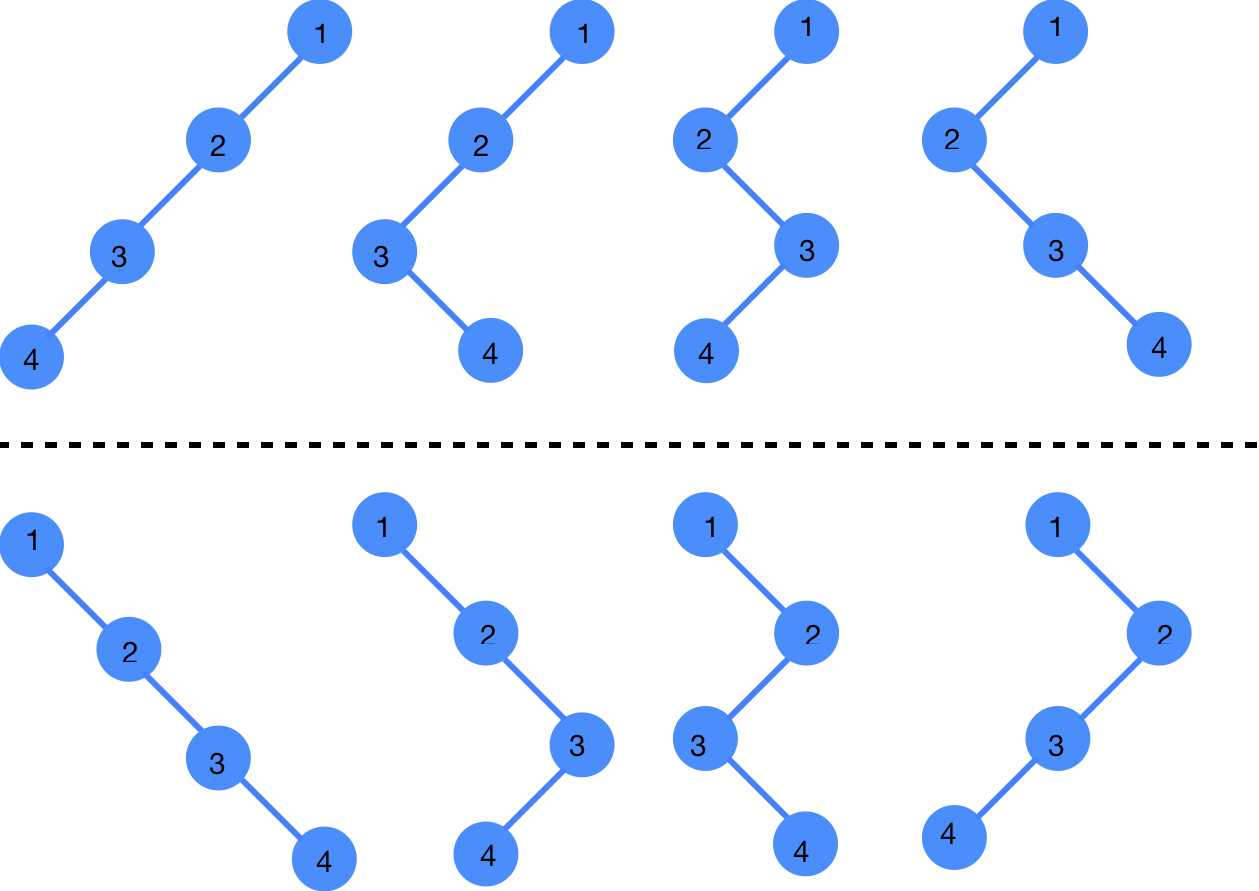
\includegraphics[scale=0.2, width=\textwidth]{4_Toppen}
\centering
\end{figure}

\begin{figure}[h]
\caption{semisplay}
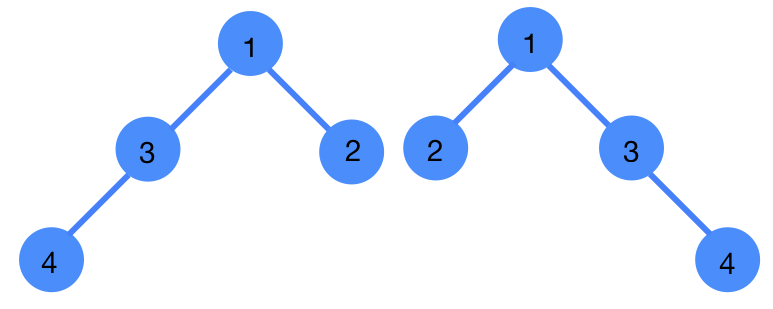
\includegraphics[scale=0.2, width=\textwidth]{4_Toppen_Semi}
\centering
\end{figure}

\begin{figure}[h]
\caption{Splaygrootte 7}
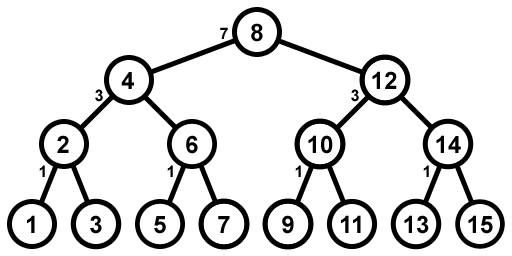
\includegraphics[scale=0.2, width=\textwidth]{Vraag2_C}
\centering
\end{figure}
\end{document}
